%///////////////////////////////////////////////////////////////////////////////
% <file>
%
% <license>
%   See the src/README.txt file for this module for copyright and license
%   information.
% </license>
%   <description>
%     <abstract>
%       This is the Webnucleo Report describing the boson condensate examples.
%     </abstract>
%     <keywords>
%       libstatmech Module, webnucleo report
%     </keywords>
%   </description>
%
%   <authors>
%     <current>
%       <author userid="tyu" start_date="2009/08/18" />
%     </current>
%     <previous>
%     </previous>
%   </authors>
%
%   <compatibility>
%     TeX (Web2C 7.4.5) 3.14159 kpathsea version 3.4.5
%   </compatibility>
%
% </file>
%///////////////////////////////////////////////////////////////////////////////
%
% This is a sample LaTeX input file.  (Version of 9 April 1986)
%
% A '%' character causes TeX to ignore all remaining text on the line,
% and is used for comments like this one.

\documentclass[pdftex]{article}    % Specifies the document style.

\usepackage[dvips]{graphicx}
\usepackage{hyperref}

                           % The preamble begins here.
\title{Webnucleo Technical Report: Boson Condensate Calculations with libstatmech}  % Declares the document's title.

\author{Tianhong Yu and Bradley S. Meyer}

\begin{document}           % End of preamble and beginning of text.

\maketitle                 % Produces the title.


This technical report describes some details of the Bose-Einstein examples
in the libstatmech distribution.

\section{Bose-Einstein Condensate}

At low temperature or high number density, a boson gas tends to collapse into
the lowest quantum state (ground state), which is a Bose-Einstein condensate.
To calculate thermodynamic quantities in this situation, we need to add the
ground state function to the integral and set the integral lower limit to 
the first excited state energy. These examples demonstrate how to add an 
user-supplied thermodynamic function and how to set a new integral lower limit.

For our system, we consider ideal bosons in
a box with sides of equal length $L$ and volume
$V = L^3$.  The single-particle states for the bosons are plane waves with
momentum ${\vec p} = 2\pi\hbar {\vec n}/L$, where ${\vec n}$ is a vector
whose components $n_x, n_y$, and $n_z$ are 0 or $\pm$integers.  The ground
state thus has momentum zero, and we consider the energy to be that less the
rest mass energy.  We may derive the thermodynamic quantities from the grand
canonical potential (see, for example, \cite{PitaevskiiAndStringari})
\[
\Omega = k_BT\sum_r \ln\left(1 - e^{\beta(\mu' - \epsilon_r')}\right),
\]
where $k_B$ is Boltzmann's constant, $T$ is the temperature, 
$\beta = 1/k_BT$, $\mu'$ is the chemical potential less the rest mass,
$\epsilon_r'$ is the energy of the single-particle state $r$ less the rest
mass, and the sum runs over all single-particle states $r$.  Since we assume
uniform density over volume $V$, the number density is given by
\[
n = -\frac{1}{V}\frac{\partial \Omega}{\partial \mu'}.
\]
By considering
all single-particle states $r$ such that $\epsilon_r = 0$, we thus find the
ground-state number density:
\[
n_0 = \frac{g}{V} \frac{1}{{\exp}(-\alpha)-1}
\]
where $g$ is the boson particle's multiplicity
and $\alpha = \mu'/kT$, which
is always negative.  The entropy density is given by
\[
s = -\frac{1}{V}\frac{\partial \Omega}{\partial T};
\]
hence, the ground-state entropy density is
\[
s_0 = -k_B \frac{g}{V}\left[
  \ln\left( 1 - e^\alpha \right )
  + \frac{\alpha}{e^{-\alpha} - 1 }
\right].
\]
Finally, the pressure is
\[
P = -\Omega / V;
\]
hence, the ground state pressure is
\[
P_0 = -\frac{k_BT}{V} g \ln\left( 1 - e^\alpha \right ).
\]
Since the ground state single-particle energy is zero and the particles are
considered to be non-interacting, the energy density of the ground state is
zero.

The boson condensate 
examples in the libstatmech distribution include these
functions, which are then set by the API routine
Libstatmech\_\_Boson\_\_updateQuantity().
Once the functions are set, they are applied during quantity calculations.

\section{Integral Lower Limit}

The non-condensate part of thermodynamic quantity calculations are still
computed with the default integrands.
Since the ground state quantities are now calculated separately, however,
we need to set
the integral lower limit to the first excited state energy over $k_BT$.  We
do this by considering the particle in this state to be non-relativistic:

\[
E_1 = \frac{p^2}{2m} = \frac{\hbar^2(2\pi/\lambda)^2}{2m} = \frac{2(\hbar\pi)^2}{mV^{2/3}}
\]

\[
x_1 = E_1/kT = \frac{2(\hbar\pi)^2}{mV^{2/3}kT}
\]

The new integral lower limit is set in the examples with the API
routine Libstatmech\_\_Boson\_\_updateIntegralLowerLimit().

\section{Results}

We may use the boson example codes in the libstatmech distribution to explore
Bose-Einstein condensation in some detail.  The examples use both
the ground-state boson functions defined above and the default integrands
with the lower integral limit $x_1$.  For example,
with the function and the integral together the number density is:

\[
n = \frac{g}{V} \frac{1}{{\exp}(-\alpha)-1}
  + \frac {(kT)^3g} {2\pi^2(\hbar c)^3}
  \int_{x_1}^{\infty}
  \frac {(x+\gamma)\sqrt{x^2+2\gamma x}} {{\exp}(x-\alpha)-1}
  \, dx
\]

When $\alpha$ (the chemical potential less rest mass over $kT$) is a large
negative number, the function term is small compared to the integral and 
is negligible.  When $\alpha$ is increasing toward zero, the
function term starts to dominate. At this point almost all the particles will
collapse into the ground state. This happens at low temperatures or high number
densities.  Figures \ref{fig:fix_T} and \ref{fig:fix_n}
below show results from the distribution examples
for a system volume $V = 1$ cm for a boson with multiplicity $g = 3$ and
a rest mass of $m c^2 = 1$ MeV.  Figure \ref{fig:fix_T} shows
the ratio of the number of particles $N_0$ in the ground state relative
to the total number of particles $N$ as a function
of the total number density of particles in the box of volume $V$.  Since
the temperature and volume are fixed, it is clear that adding particles to
the system eventually causes condensation in which most of the particles
are in the ground state.  The number density at which condensation occurs
increases for higher temperature because the probability to excite a given
boson to the first excited state is higher for higher $T$.

\begin{figure}[htp]
\centering
\resizebox{\textwidth}{!}{
  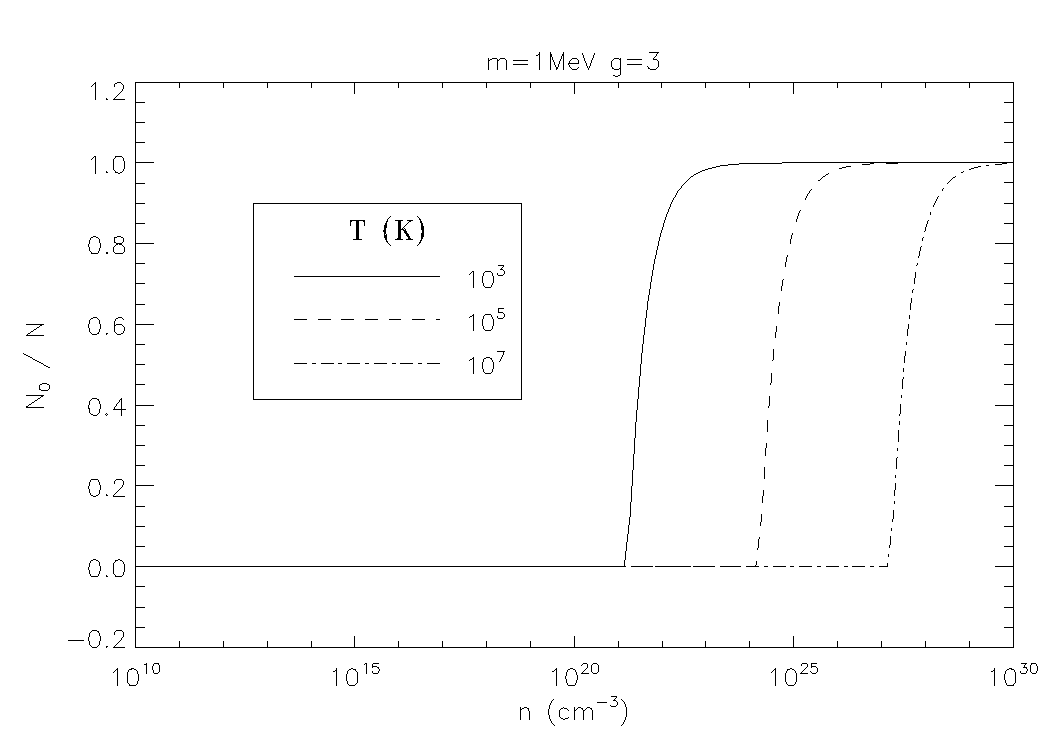
\includegraphics{figures/fix_T}
  }
\caption{Ground state fraction vs number density at different temperatures.
  $N_0$ is the number of particles in the ground state, while $N$ is the
  total particle number.}
\label{fig:fix_T}
\end{figure}

Condensation also occurs when the temperature is lowered for fixed number
density.  Figure \ref{fig:fix_n} shows this for several number densities.
As the temperature is lowered, a temperature is reached at which the fraction
of particles in the ground state rises quickly.  This is the phase
transition to the condensate.

\begin{figure}[htp]
\centering
\resizebox{\textwidth}{!}{
  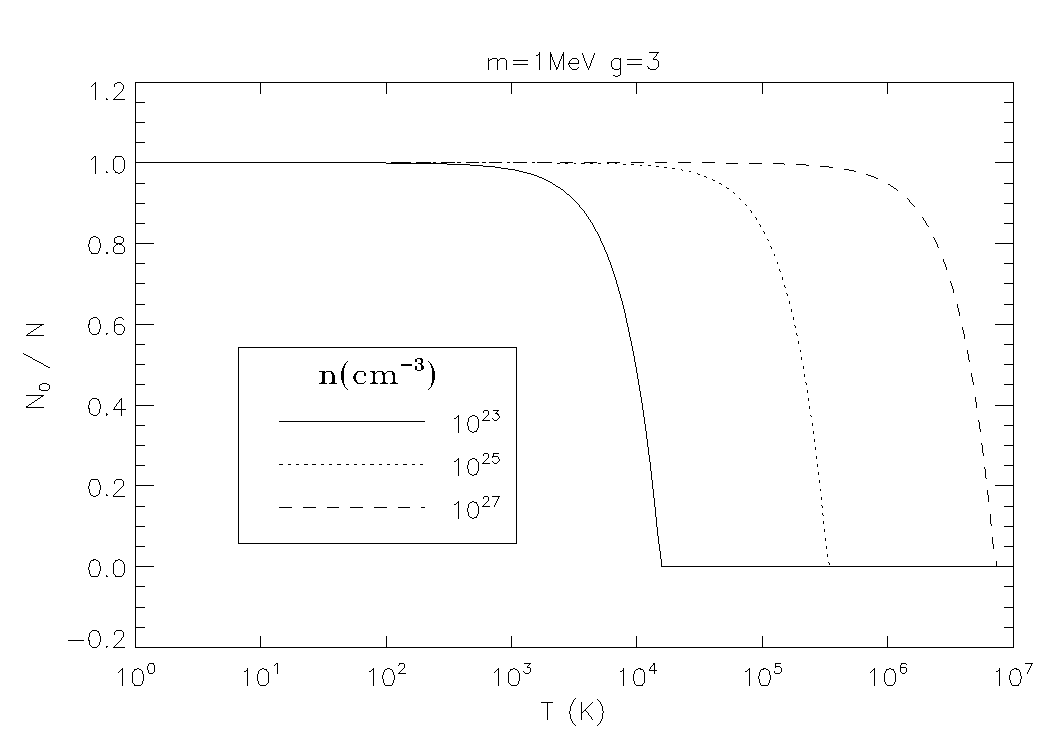
\includegraphics{figures/fix_n}
  }
\caption{Ground state fraction vs temperature at different number densities.
  $N_0$ is the number of particles in the ground state, while $N$ is the
  total particle number.}
\label{fig:fix_n}
\end{figure}

The critical temperature $T_c$ at which the phase transition occurs may
be computed for non-relativistic bosons to be
\[
T_c = \frac{2\pi\hbar^2}{mk_B}\left(\frac{n}{g\zeta(3/2)}\right)^{2/3},
\]
where $\zeta(3/2)$ is the Riemann zeta function of argument 3/2
\cite{PitaevskiiAndStringari}.  Figure \ref{fig:n_tc} shows $N_0 / N$ as
a function of $T/T_c$ as computed with a libstatmech example code.  It
is clear that condensation does indeed occur at $T_c$.  Figure \ref{fig:cv}
shows the specific heat capacity as a function of $T/T_c$ as computed from
a libstatmech example code with $g = 3$ and $mc^2 = 100$ MeV.
The cusp in the curve at $T = T_c$ is the signal of the phase transition.
As $T$ increases above $T_c$, the specific heat capacity settles down
towards $3k_B/2$, as expected for a non-relativistic, ideal gas.

\begin{figure}[htp]
\centering
\resizebox{\textwidth}{!}{
  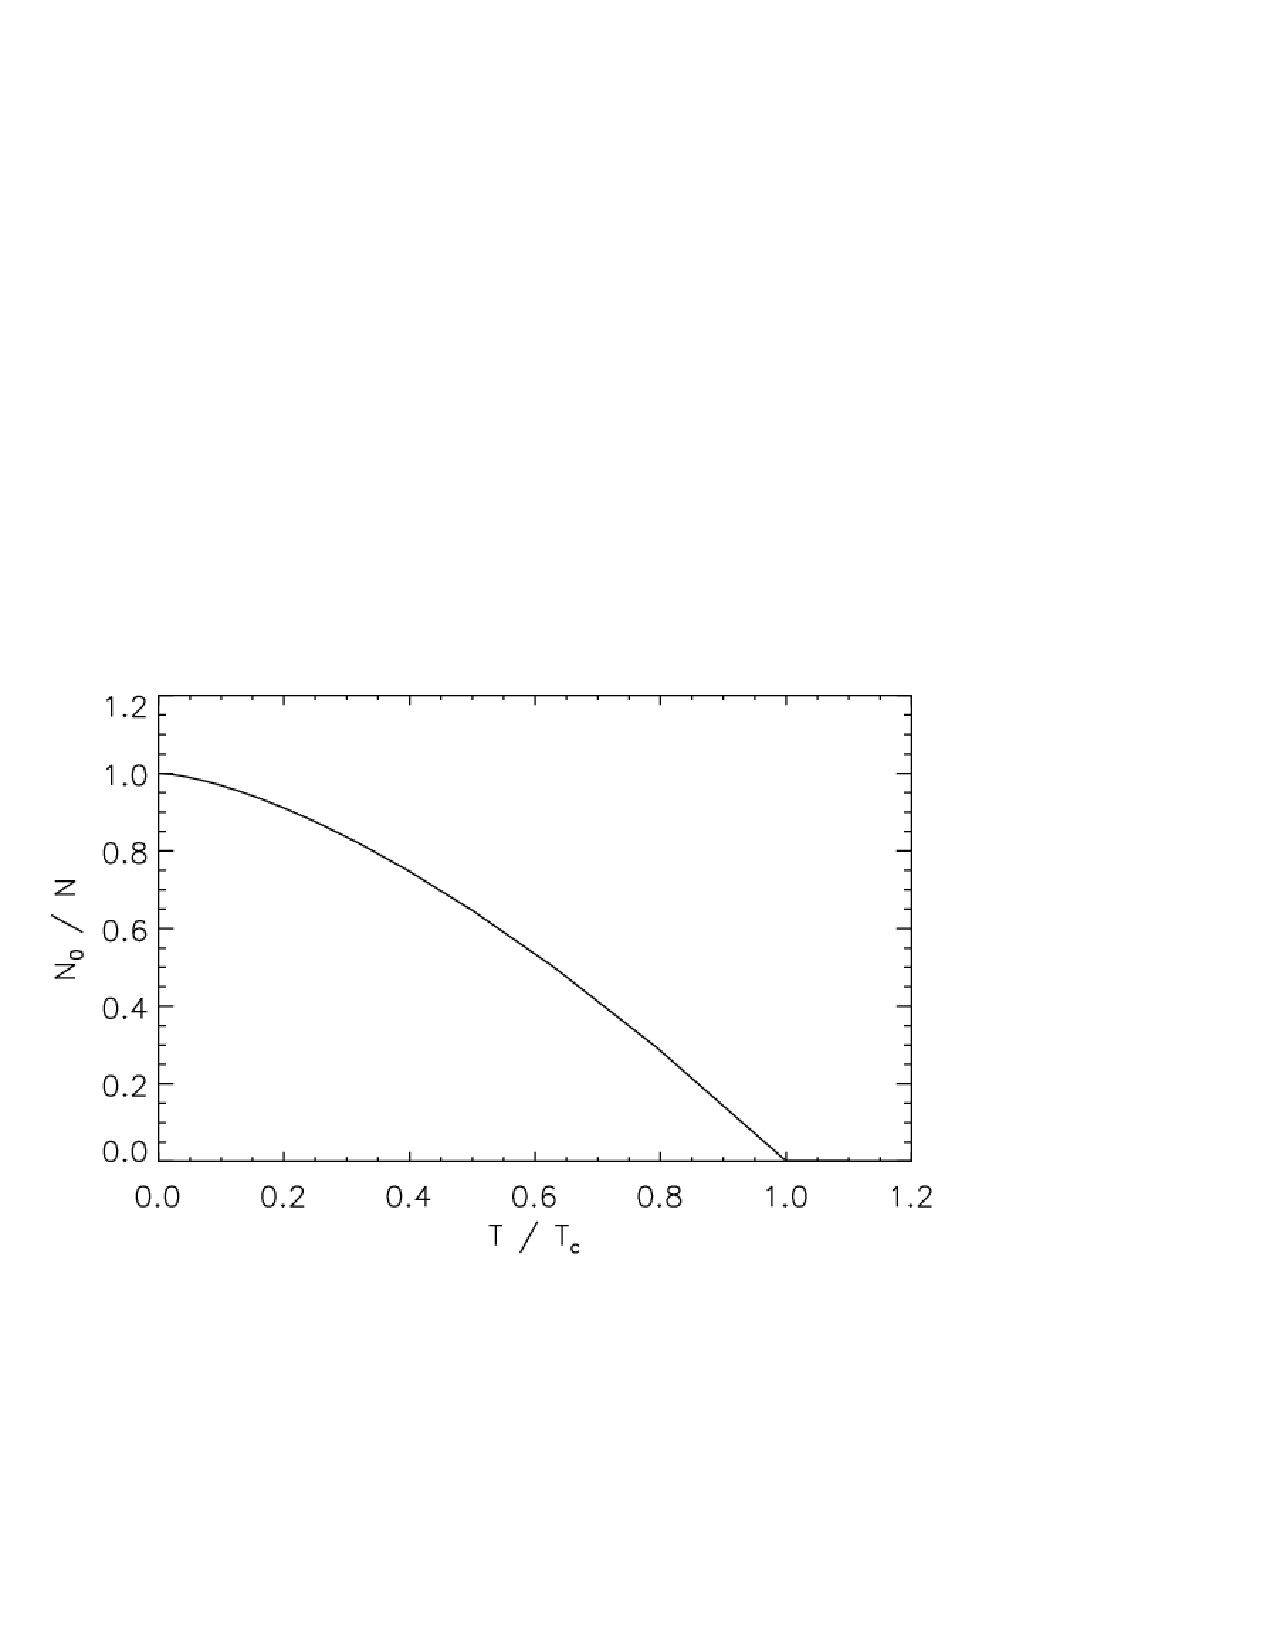
\includegraphics{figures/bec_n_n}
  }
\caption{Ground state fraction as a function of the temperature relative
  to the critical temperature for an ideal boson gas with $mc^2 = 100$ MeV
  and $g = 3$.}
\label{fig:n_tc}
\end{figure}

\begin{figure}[htp]
\centering
\resizebox{\textwidth}{!}{
  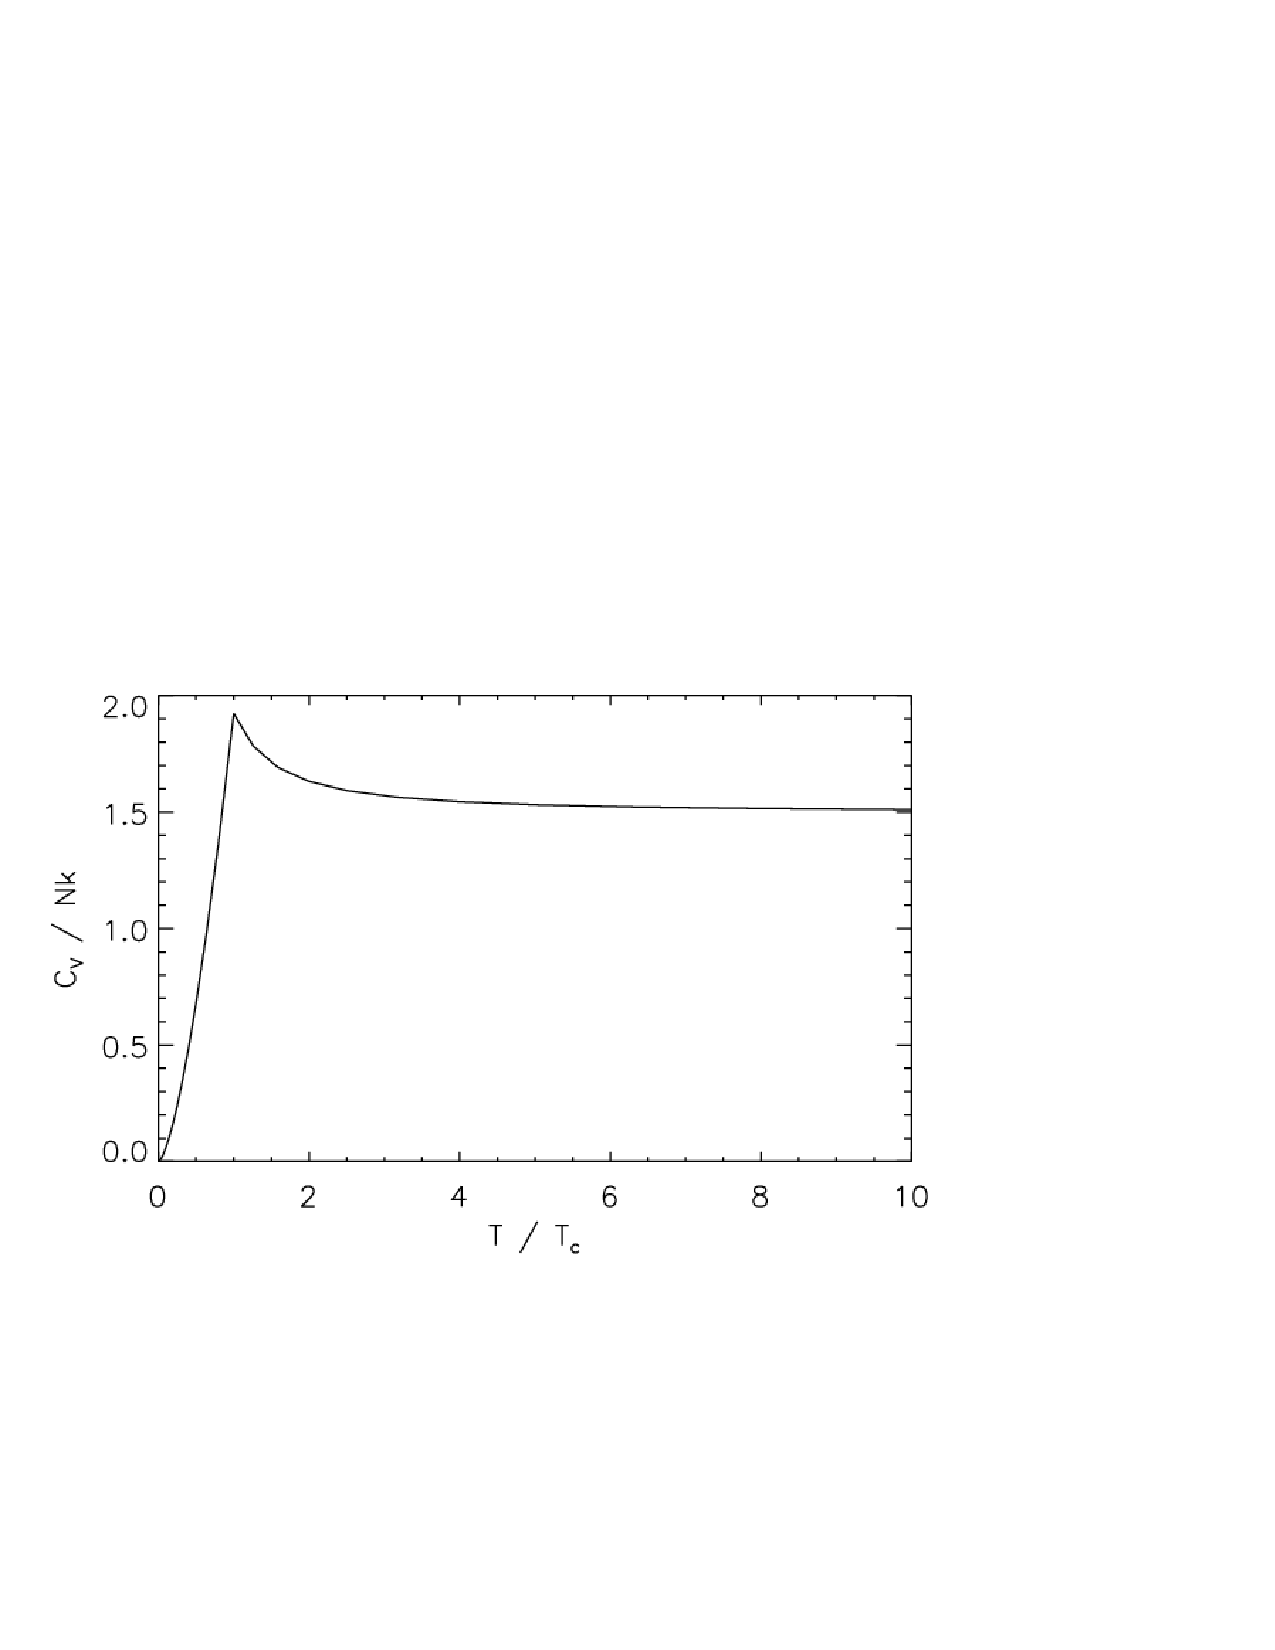
\includegraphics{figures/bec_n_cv}
  }
\caption{
Specific heat capacity as a function of temperature for the ideal boson
gas.
}
\label{fig:cv}
\end{figure}

Figure \ref{fig:bec_p} shows the pressure of an ideal boson gas with
$mc^2 = 100$ MeV and $g = 3$ as a function of the number density for a
fixed temperature of 100 K.  Below the condensation, the pressure is
proportional to the number density, as expected for an ideal, non-relativistic
gas.  Once the number density exceeds the critical number density,
the pressure becomes constant as a function of number density.  This
surprising result is due to the fact that, as the number of particles
increases towards infinity, the number of particles not in the ground
state becomes a constant.  To understand this, consider a two-state system
with a probability $p$ for a single particle not to be in the ground state.
The particles are indistinguishable; therefore, the probability to have $m$ out of a
total of $N$ particles not in the ground state is $P(m) = {\cal N} p^m$,
where ${\cal N}$ is a normalization constant.  This means
that
\[
{\cal N} \sum_{m=0}^N p^m = 1.
\]
If $N \to \infty$, then ${\cal N} = 1 - p$.  The total number of particles not
in the ground state for large $N$ is thus
\[
\sum_{m>0} (1 - p) m p^m = (1 - p) p \frac{d}{dp} \sum_{m=0} p^m = (1 - p) p / (1 - p)^2 = p / (1 - p).
\]
This becomes a negligible fraction of $N$ as $N \to \infty$.  Nevertheless,
it is these particles that carry the energy, pressure,
and entropy; hence, these quantities become constant as a function of
the number density when the condensation occurs.

\begin{figure}[htp]
\centering
\resizebox{\textwidth}{!}{
  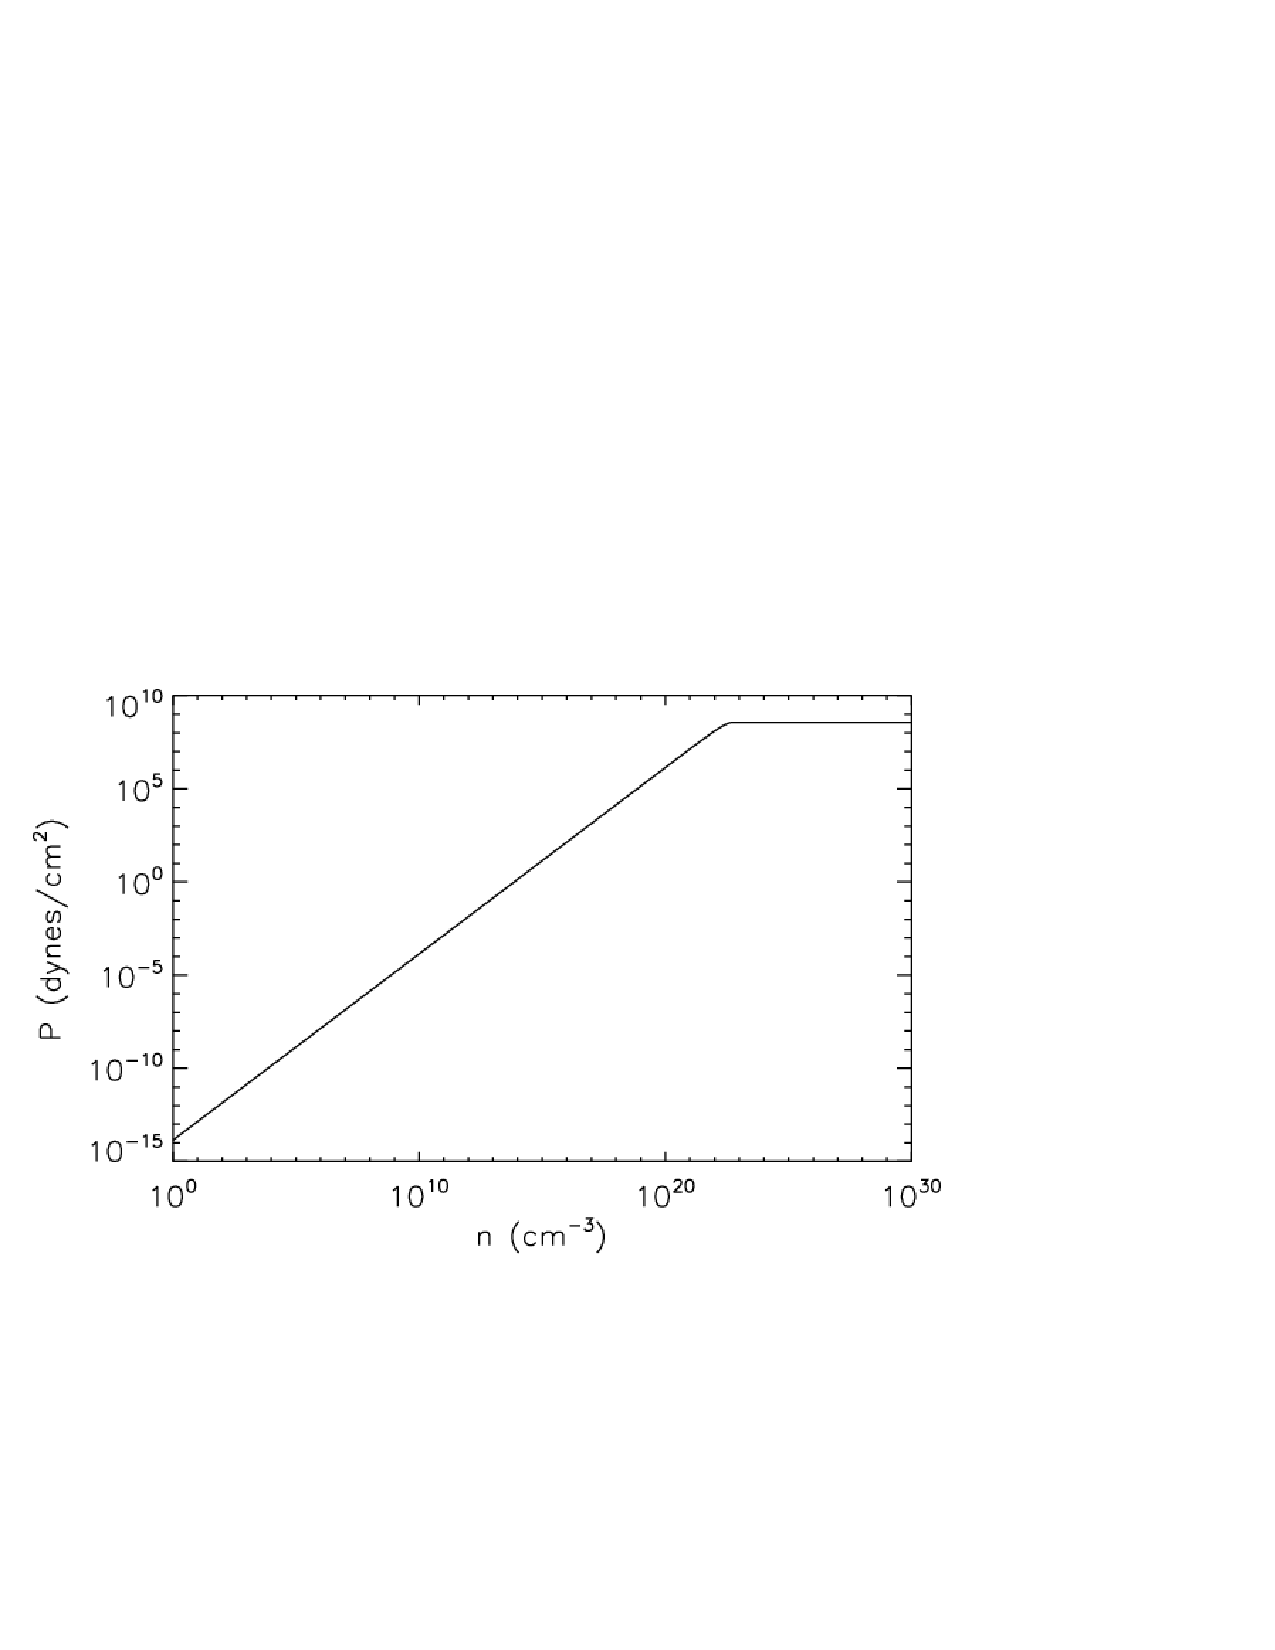
\includegraphics{figures/bec_T_p}
  }
\caption{
Pressure as a function of number density for an ideal gas of bosons
with mass $mc^2 = 100$ MeV and $g = 3$ at $T = 100$ K.  Once condensation
occurs, the pressure is independent of the number density.
}
\label{fig:bec_p}
\end{figure}

\bibliographystyle{siam}

\begin{thebibliography}{1}

\bibitem{PitaevskiiAndStringari}
{\sc L.~{Pitaevskii} and S.~{Stringari}}, {\em {Bose-Einstein Condensation}},
  Oxford University Press, New York, NY, 2003.

\end{thebibliography}

\end{document}
